%%%%%%%%%%%%%%%%%%%%%%%%%%%%%%%%%%%%%%%%%%%%%%%%%%%
%
%  New template code for TAMU Theses and Dissertations starting Fall 2012.
%  For more info about this template or the
%  TAMU LaTeX User's Group, see http://www.howdy.me/.
%
%  Author: Wendy Lynn Turner
%	 Version 1.0
%  Last updated 8/5/2012
%
%%%%%%%%%%%%%%%%%%%%%%%%%%%%%%%%%%%%%%%%%%%%%%%%%%%
%%%%%%%%%%%%%%%%%%%%%%%%%%%%%%%%%%%%%%%%%%%%%%%%%%%%%%%%%%%%%%%%%%%%%%
%%                           SECTION III
%%%%%%%%%%%%%%%%%%%%%%%%%%%%%%%%%%%%%%%%%%%%%%%%%%%%%%%%%%%%%%%%%%%%%



\chapter{\uppercase{Results and Conclusions}}

Each language had it's own advantages and disadvantages to the ray tracing process.  These were futher accentuated by the speed tests conducted for each Milestone.  The results for each speed test were to be as expected from common knownledge of each language, and from more rigourous tests conducted by other computer scientists.  Python was the slowest by far, with Processing holding the middle ground and C++ being the fastest.  Surprisingly however, the speed difference between Process and C++ is less than what might have been expected, since C++ is compiled before running the test and Processing's speed test is considered with the processing ``play'' button.  

\section{Conclusions}
Each language will be discussed with it's pro's and con's and at the end of this section a reccomendation will be made as to the most suitable language that might maximize focus on the implementation theory rather than the implementation process of writing code syntax.  It can be established as a baseline for all languages however that you MUST learn a certain baseline of scripting and coding concepts. Language syntax and compilation processes cannot be avoided.  

\subsection{C++}
C++ is the fastest processor of all the languages tested.  This allowed for quicker iterations and more creative freedom with the final images because of the quick process speed.  C++ was able to process the scale of computation for large images far quicker that either Java or Python.  However, C++ is not an easy language to learn.  There was much more overhead to learn in order to compile and set up an C++ project.  Whereas in the other languages you just needed to learn how to create a executable file and run that within the correct environment, c++ had a variety of compilers to choose from, and then a multitude of files and commands to run before the image would appear on the screen.  This could be automated to save time, but the initial process to a new programmer is not intuitive to quickly write and execute a ray tracer.  However, having written the first ray tracer in c++, which exposes the basic process of how a computer handles executing a program, since with c++ you need to ``make'' and then run the program, this intuitively allowed the implementation of the other ray tracers to go faster.  However, since practically most artists will be writing only one ray tracer, the knowledge of how to compile and run the program still needs to be accomplished, but is less forgiving or intiutive with c++.

\subsection{Processing}
Processing was the easiest to compile and execute code.  Processing has expedited this process by packaging the code compiler within it's own custom ``API'' (processing the language for this thesis encompasses both the java language and the processing executable that is delivered with a download of Processing).  While Processing comes with a the neccesary libraries to implement a ray tracer, using these introduces another challenge.  Addition in this language with the supplied Vector form was done through a function(Vector.add()) rather than through an operator (such as plus ``+'' or minus ``-'').  While unintuitive for complex math functions, over all this was a small setback in creating a raytracer.  The benefits of an expedited compilation process out weighs the intial difficulty of figuring out language syntax.

\subsection{Python}
Python was the slowest of all the languages test.  However, it was the easiest to write code in.  While there are still rules to follow when creating Python code, as there are in C++ or in Processing, there are far less of them.  Since Java and C++ are both statically typed, they need more strict rules as to when variables can be set and what those variables can be set as.  A lot of time was spent learning and understanding polymorphism and subtyping for Java and C++ so that each ray tracer can more closely mimic the ray tracing theory.  With Python, none of this research was necessary in order to accomplish these complex data structures.  However Python was significantly slower than both Python and Processing.  While this means Pixar or Dreamworks will not be using Python for their next iteration of their ray tracer, for learning ray tracing theory this was of no consequence.  When establishing a workflow to create a python image, a lower resolution ``layout'' was used to prepare a final render, instead of testing images with the full resolution everytime.  

%%%%%%%%%%%%%%%%%%%%%%%%%%%%%%%%%%%%%%%%%%%%%%%%%%%%%%
\begin{figure}[H]
\centering
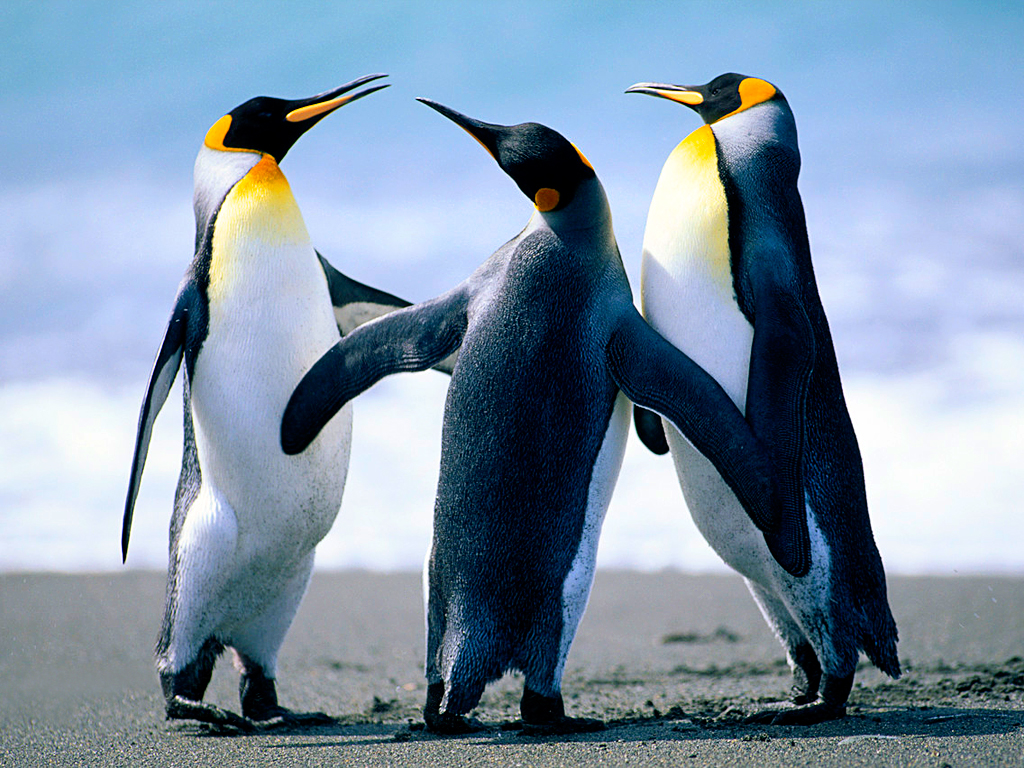
\includegraphics[scale=.50]{figures/Penguins.jpg}
\caption{TAMU figure}
\label{fig:tamu-fig3}
\end{figure}
%%%%%%%%%%%%%%%%%%%%%%%%%%%%%%%%%%%%%%%%%%%%%%%%%%%%%%
\section{Another Section}

Text between the figures.  Text between the figures. Text between the figures. Text between the figures.  Text between the figures. Text between the figures. Text between the figures.  Text between the figures. Text between the figures. Text between the figures.  Text between the figures. Text between the figures.
%%%%%%%%%%%%%%%%%%%%%%%%%%%%%%%%%%%%%%%%%%%%%%%%%%%%%%%
%\begin{figure}[H]
%\centering
%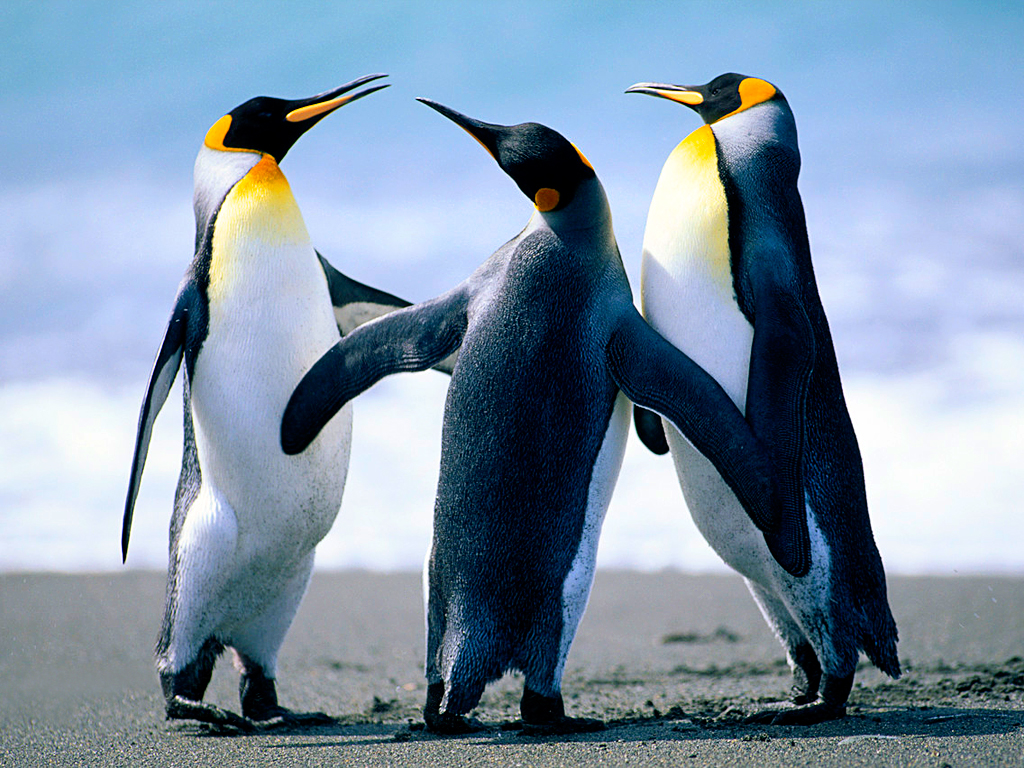
\includegraphics[scale=.50]{figures/Penguins.jpg}
%\caption{Another TAMU figure}
%\label{fig:tamu-fig4}
%\end{figure}
%%%%%%%%%%%%%%%%%%%%%%%%%%%%%%%%%%%%%%%%%%%%%%%%%%%%%%%

\subsection{Subsection}

%%%%%%%%%%%%%%%%%%%%%%%%%%%%%%%%%%%%%%%%%%%%%%%%%%%%%%%
%\begin{figure}[H]
%\centering
%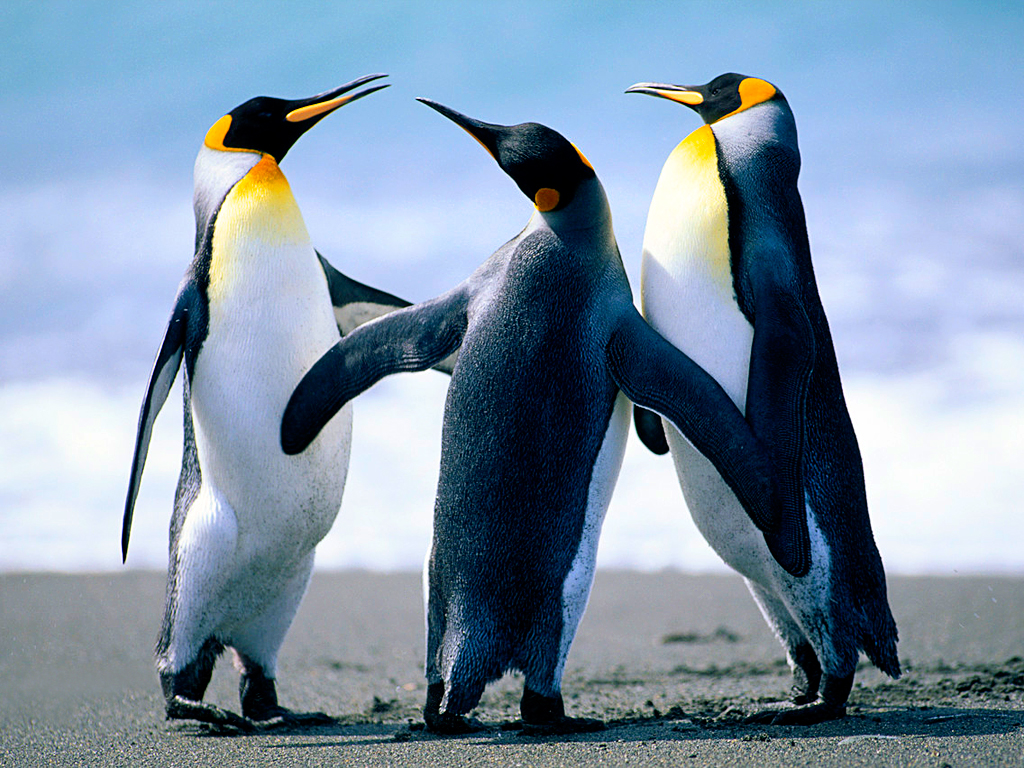
\includegraphics[scale=.50]{figures/Penguins.jpg}
%\caption{Another TAMU figure}
%\label{fig:tamu-fig4-2}
%\end{figure}
%%%%%%%%%%%%%%%%%%%%%%%%%%%%%%%%%%%%%%%%%%%%%%%%%%%%%%%
\subsection{Subsection}

A table example is going to follow.

\begin{table}[H]
\centering
\caption{This is a table template}
\begin{tabular}{|l|c|c|c|c|c|}
\hline
Product & 1 & 2 & 3 & 4 & 5\\
\hline
Price & 124.- & 136.- & 85.- & 156.- & 23.-\\
Guarantee [years] & 1 & 2 & - & 3 & 1\\
Rating & 89\% & 84\% & 51\% & & 45\%\\
\hline
\hline
Recommended & yes & yes & no & no & no\\
\hline
\end{tabular}
\label{tab:template2}
\end{table}
\section{Another Section} 